\documentclass[10pt, conference, compsocconf]{IEEEtran}
\usepackage[T1]{fontenc}
\usepackage[utf8]{inputenc}
\usepackage[brazilian]{babel}
\usepackage{verbatim}
\usepackage{scalefnt}
\usepackage{xcolor}
\usepackage{ulem}
\usepackage{type1cm}
\usepackage{url}
\usepackage{subfigure}
\usepackage{courier}
\newcommand{\TODO}[1]{{\color{red}\textbf{\uwave{#1}}}}

\usepackage[pdftex]{graphicx}
\DeclareGraphicsExtensions{.png}

\title{Kalibro Metrics: a multi-repository and multi-language source
code analysis tool}

\author{
	\IEEEauthorblockN{Carlos Morais$^1$, Paulo Meirelles$^1$, Vin\'icius Daros$^1$, Fabio Kon$^1$}
	\IEEEauthorblockA{
		$^1$Department of Computer Science\\
		Institute of Mathematics and Statistics\\
		University of S\~ao Paulo, Brazil\\
		\{morais, paulormm, vkdaros, fabio.kon\}@ime.usp.br
	}
	
\and

	\IEEEauthorblockN{Carlos Santos Jr.$^1$$^,$$^2$}
	\IEEEauthorblockA{
		$^2$Horizon Institute\\
		University of Nottingham, United Kingdom\\
		carlos.denner@nottingham.ac.uk
	}

}

%-------------------------------------------------------------------------------
\begin{document}
\normalem
\def\UrlFont{\tt\footnotesize}
\maketitle

\begin{abstract}

Neste texto apresentamos os resultados intermediários de um Trabalho de Conclusão de Curso de Engenharia de Software da UnB. Assim, é explorada a importância da utilização de métricas estáticas de código-fonte para suportar a tomada de decisões, tanto a nível técnico quanto gerencial a respeito do \emph{design} e segurança do software. Além disso, é proposta uma nova técnica para realizar medições que será viabilizada a partir da evolução de duas ferramentas de monitoramento de código-fonte.

\end{abstract}
\vspace{1\baselineskip}

\begin{keywords}
Métricas; Design; Segurança; Monitoramento; Cenários de Decisões; Código-fonte;
\end{keywords}





\IEEEpeerreviewmaketitle

%-------------------------------------------------------------------------------

\section{Introdução}
\label{introduction}

A qualidade interna é um dos fatores de sucesso de projetos de software, pois corresponde à aspectos como manutenibilidade e segurança. Softwares com boa qualidade interna proporcionam maior produtividade uma vez que possibilitam a criação de mais testes automatizados, são mais compreensíveis, reduzem o risco de \emph{bugs} e facilitam as modificações e evoluções no código.
%
Além disso, um estudo do ICAT/NIST
%
\footnote{ICAT foi um motor de busca de vulnerabilidades, desenvolvido pelo NIST(National Institue of Standards and Technology), catalogadas no padrão \emph{Common Vulnerabilities and Exposures} - CVE. O ICAT foi substituido pelo NVD (National Vulnerability Database) que, além de possuir o mesmo mecanismo de busca, é um repositório governamental dos Estados Unidos que armazena diversas informações sobre vulnerabilidades de software (nomenclaturas, métricas, checklists, etc).}
%
de 2005 já apontava que 80\% das vulnerabilidades exploráveis estão ligadas a má codificação.

Nesse sentido, a medição pode ser utilizada como um processo de apoio ao acompanhamento da segurança e qualidade, através do estabelecimento de metas e indicadores que indiquem oportunidades de melhorias observáveis do produto. Em um cenário otimista,
os próprios Engenheiros de Software podem adotar como prática a medição do código-fonte para auxiliar as tomadas de decisões, ou até mesmo para avaliação do código inserido ou da aplicação de refatorações. Entretanto, uma grande quantidade de métricas, coletas manuais e poucos recursos de visualização são fatores que acabam por desmotivar o uso dessas para o monitoramento do código. Além disso, assim como destacado por \cite{chidamber1994}, a compreensão do significado de valores obtidos através de métricas não é uma tarefa trivial, demandando um grande esforço de coleta e interpretação, cujas análises podem ser errôneas caso feitas sobre métricas isoladas, correlações inexistes ou até mesmo a escolha de métricas inadequadas.

Nesse contexto, métricas de código-fonte podem ser utilizadas tanto no âmbito gerencial quanto como referência técnica para tomada de decisões sobre o código-fonte. Métricas de código-fonte possuem natureza objetiva que buscam mensurar tamanho, complexidade e outros atributos importantes do software \cite{henry1984kafura}\cite{troy1981zweben}\cite{yau1985zweben}\cite{systa2000}. Neste sentido, o estudo de métricas e sua utilização no contexto de segurança e qualidade interna do código-fonte podem ser fundamentais para a formação do Engenheiro de Software.

Neste artigo, iremos mostrar os estudos e resultados intermediários de um trabalho de conclusão de curso de Engenharia de Software da Faculdade UnB Gama, cujo foco é explorar e potencializar a utilização de métricas para o monitoramento de código-fonte a partir da compreensão e estabelecimento de possíveis relações existentes entre métricas de vulnerabilidade e qualidade de software. Assim, esse trabalho contempla a composição de métricas em cenários de decisões e o desenvolvimento e evolução de duas ferramentas que possam apoiar a utilização de métricas e cenários na melhoria contínua do desenvolvimento. A primeira ferramenta consiste em uma plataforma livre de monitoramento de código fonte chamada Mezuro, enquanto a segunda consiste em um ambiente de \emph{Data Warehousing} que também já foi explorado em outros trabalhos \cite{Folleco2007}\cite{Silveira2010}\cite{mazuco2011}.

No presente texto iremos apresentar na Seção \ref{sec:methodology} como foi nossa organização e metodologia utilizada durante a execução do trabalho de conclusão de curso. Posteriormente, a Seção \ref{sec:studies} apresenta os estudos e resultados obtidos até o momento no trabalho. Por fim, a Seção \ref{sec:final-remarkds} conclúi este artigo e mostra os trabalhos futuros.


\section{Projeto}
\label{sec:projeto}


O Portal do Software Público Brasileiro, SPB, inaugurado em 2007, na prática, é um sistema
web que se consolidou como um ambiente de compartilhamento de projetos de software.
Oferece um espaço (comunidade) para cada software. A comunidade é composta por fórum,
notícias, chat, armazenamento de ae rquivos e downloads, wiki, lista de prestadores de
serviços, usuários, coordenadores, entre outros recursos. Teve um crescimento expressivo
contando, hoje, com mais de 60 comunidades de desenvolvimento e mais de 200.000 usuários
cadastrados. O SPB abrange também, o 4CMBr que é o grupo de interesse voltado para
soluções de tecnologia para municípios, o 5CQualiBr que é um grupo que trabalha para
evoluir a qualidade do Software Público Brasileiro, o 4CTecBr, um portal destinado a
colaboração no desenvolvimento de Tecnologias Livres, o Mercado Público Virtual que é um
grupo de empresas e pessoas que prestam serviço nos softwares ofertados no Portal e o Ava- 
liaSPB que avalia a entrada dos softwares candidatos a software público. O ambiente do 
SPB não proporciona a integração com ambientes colaborativos externos, especialmente com
redes sociais. A plataforma escolhida na ocasião da criação foi o framework OpenACS, que
continua sendo utilizada na atual versão.
%
A evolução do SPB foi comprometida desde 2009, quando framework OpenACS foi 
descontinuado. Com isso, não tendo versões lançadas a partir daquele ano. Por isso, hoje,
é necessária a evolução para novas tecnologias, que tenham maior suporte das comunidades
de desenvolvimento, utilize linguagens de programação com maior velocidade de
desenvolvimento e permita a integração com ambientes colaborativos externos, em especial,
redes sociais. Além disso, é preciso realizar a manutenção evolutiva das funcionalidades
existentes e também o desenvolvimento de novas funcionalidades para o Portal do SPB .
%
Um dos passos para a concretização de uma nova geração do Portal SPB é a integração de
novas tecnologias, desde uma plataforma colaborativa até sistemas de controle de versão e
monitoramento da qualidade do código-fonte, gerenciadas e apresentadas em uma plataforma
integrada no back-end e, em especial, no front-end para que os usuários e as comunidades
dos projetos tenham um conjunto de recursos para encontrarem os projetos, bem como
colaborarem em torno de um sofware público.
%
Mesmo com as limitações citadas, o Portal do Software Público Brasileiro teve em 2013 
mais de 600 mil visitantes únicos, com mais de 1 milhão de visitas/acessos, gerando mais
de 16 milhões de visitadas nas páginas, com um total de mais de 49 milhões de hits no
Portal SPB. Avaliando apenas as comunidades dos projetos I3Geo, CAU, CACIC e Geplanes,
houve mais de 15 mil downloads e 4 mil mensagens nos fórum. Essa amostra estatística
ilustra bem o potencial do Software Público Brasileiro, bem como as expectativas de seus
usuários e colaboradores para a evolução do Portal e do modelo em si.

\section{Arquitetura}
\label{sec:arquitetura}

O sistema que irá atender a evolução e reformulação do Portal do Software Público Brasileiro constitui-se de diversos módulos e que irão comunicar-se entre si de forma organizada e integrada para suprir as necessidades do projeto.
%

\begin{figure}[htpb]
  \begin{center}
    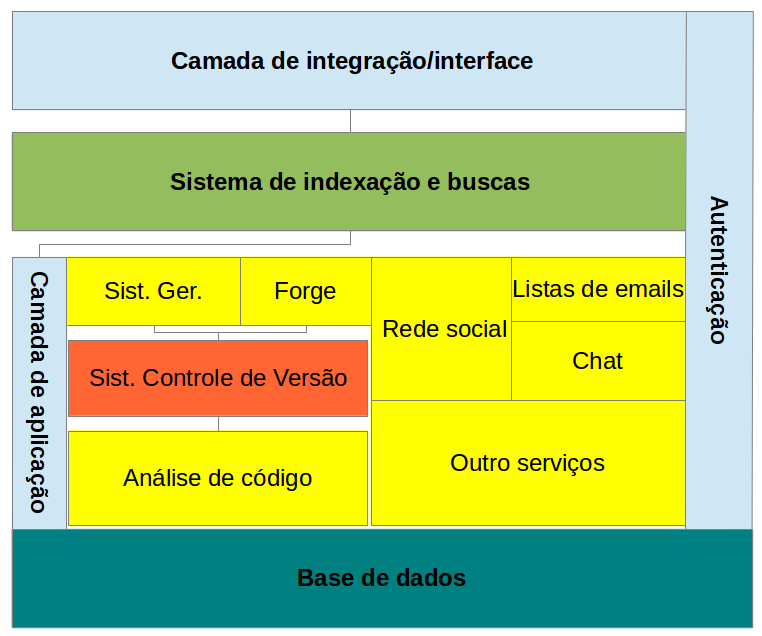
\includegraphics[width=.37\textwidth]{images/visao_arq.png}
  \end{center}
  \caption{Proposta de arquitetura do Novo Portal do Software Público}
  \label{fig:core_concurrent}
\end{figure}
%\vspace{-0.5em}

As ferramentas que serão utilizadas para suprir essas necessidades serão:

\begin{itemize}

\item Para lista de e-mail estamos utilizando o Mailman na versão 2 que é um software gratuito para gerenciamento de discussão eletrônica de e-mail e listas e- newsletter.

\item Para Chat estamos utilizando Punjab BOSH (XMPP) que é  É uma interface HTTP cliente jabber. É um gerenciador de conexão BOSH que permite conexões de clientes persistentes para um servidor XMPP (protocolo de comunicação para mensagens orientadas a middleware baseado em XML)

\item Para Plataforma de Buscas estamos utilizando Apache Solr que é uma plataforma de busca open source da Apache Lucene escrita em Java

\item Para rede social estamos utilizando o Noosfero que é uma plataforma web livre para criação de redes sociais com blog, e-Portifólios, CMS, RSS, discussão temática, agenda de eventos, galeria de imagens, chat, entre outros. Ele foi desenvolvido pela Cooperativa de Tecnologias Livres – Colivre 3 em 2007, sob a licença AGPL v.3, com a proposta de permitir ao usuário criar sua própria rede social personalizada, livre e autônoma.

\item Para Forge para SVN estamos utilizando o Trac que é uma ferramenta open source para controle de mudança em projetos de desenvolvimento

\item Para sistemas de controle de versão estamos utilizando SVN e Git que são ferramentas open-source para controle de mudança em projetos de desenvolvimento

\item Para Forge para Git estamos utilizando o GitLab que é um software livre de colaboração de código online que utiliza a ferramenta de gerência de código-fonte Git

\item Para sistema de gerenciamento estamos utilizando o Redmine que é uma aplicação web de gerenciamento de projetos que disponibiliza diversas ferramentas para auxiliar a gestão e manutenção de um projeto

\item Para suporte a Single Sign On estamos utilizando o Mozilla Persona que foi desenvolvido pela Mozilla e permite o suporte a single sign on

\item Para Sistema de Integração contínua estamos utilizando o Jenkins que é uma aplicação web de integração contínua de construção de projetos

\end{itemize}

Para integrar todas estas ferramentas estamos utilizando o Colab que nada mais é que uma plataforma de integração de ferramentas, o qual são integradas também as interfaces das ferramentas para que ao navegar o usuário tenha a sensação de estar navegando em uma única ferramenta.

Neste projeto notamos a necessidade de utilizar vários elementos que softwares livres já oferecem e não vimos sentido em refazer algo que já está pronto e disponível para ser utilizado. No início do projeto gastamos algum tempo estudando possíveis ferramentas que pudessem ser utilizadas para resolver os diferentes problemas e para resolver e chegamos a lista apresentada.  


\section{Metodologia de Desenvolvimento}
\label{sec:metodologia}

A Engenharia de Software tem evoluído suas práticas e metodologias em busca de padrões que regem o desenvolvimento de software de qualidade dentro dos escopos, custos e prazos desejados. O modelo dito tradicional tem como característica um conjunto grande e detalhado de documentação que deve, supostamente, ser utilizada ao longo de todo o ciclo de desenvolvimento. Entretanto, percebendo que os objetivos principais do desenvolvimento de software não estavam sendo alcançados, alguns líderes da indústria e academia começaram a adotar métodos mais simples de trabalho que apresentaram melhores resultados em projetos de software. Em 2001, líderes que estavam desenvolvendo projetos fora dos padrões industriais se reuniram para trocar experiências e trabalhos. Este grupo se tornou a Aliança de Desenvolvimento Ágil e escreveram o Manisfesto Ágil que apresenta os princípios e valores que o grupo considera ser determinante para o desenvolvimento de software. Neste sentido, os métodos de desenvolvimento ágeis de software são métodos que implementam os seguintes valores:

\begin{itemize}

\item Indivíduos e interações acima de processos e ferramentas; 

\item Software operante acima de documentações grandes e completas; 

\item Colaboração do cliente acima de negociações contratuais; 

\item Responder à mudanças acima de seguir a um planejamento.

\end{itemize}

Esse conjunto de valores não descartam a importância dos elementos citados à direita das sen- 
tenças, mas evidenciam que estes são menos importantes diante dos primeiros elementos citados. 
Em outras palavras, apesar da documentação ser importante, o foco principal deve estar na entrega 
de software de valor para o cliente e na interação e a consequente comunicação entre as pessoas. 
Além disso, os métodos ágeis exaltam a simplicidade, feedback contínuo e adaptação à mudanças 
que podem ser obitidos a partir de comunicação face à face, qualidade de código e entrega contínua 
de software. 

Dada a oportunidade de adoção de métodos ágeis no desenvolvimento do presente trabalho, a 
metodologia utilizada é baseada em uma combinação das metodologias Scrum e Extreme Programming. Destacam que XP e Scrum complementam um ao outro bem, com o XP provendo suporte para aspectos mais técnicos enquanto o Scrum provê práticas e técnicas para gerenciamento, planejamento e acompanhamento. Assim,com base nas experiências destacadas em [Schwaber and Beedle, 2001] e 21 [Fitzgerald et al., 2006], na motivação de adoção de métodos ágeis no desenvolvimento de software moderno, serão apresentadas os métodos XP e Scrum, suas principais características e práticas que serão utilizadas no desenvolvimento do presente projeto.


\section{Escolha da equipe}
\label{sec:equipe}

	A equipe é formada majoritariamente por alunos de graduação do curso de Engenharia de Software da Universidade de Brasília, conta ainda com dois ex-alunos formados, alunos de mestrado que trabalham exclusivamente com o design além de professores orientadores. 
	
	Devido a esta formação a equipe não consegue estar sempre trabalhando junta pois cada um possui seu horário de aula e adéqua as horas de contribuição ao projeto a este horário de aulas, dessa forma não conseguimos utilizar os métodos ágeis na íntegra.
	
	Esta equipe maior está dividida em duas equipes menores onde uma dessas equipes está trabalhando com o Nosfero e a outra equipe está trabalhando com Colab e as integrações das demais ferramentas. A equipe do Noosfero está desenvolvendo um plugin com novas funcionalidades para o Portal do Software Público. A equipe do Colab ainda está trabalhando com configurações das ferramentas pois está sendo integrado o Redmine e o Gitlab com o Colab e está exigindo maiores esforços de infra-estrutura.
	
	Para manter o controle das atividades do projeto e evitar os ruídos de comunicação temos uma lista de e-mail com todos os integrantes do projeto, onde foi criado o hábito de enviarmos um e-mail ao final do dia com as atividades que desenvolvemos. Temos também um dia da semana em que todos estão no laboratório onde fazemos um stand up para alinharmos a situação das equipes. Utilizamos ainda o Redmine para fazer o gerenciaento do projeto, onde são escritas histórias de usuários e histórias técnicas e suas respectivas tarefas. Estamos trabalhando em sprints/ciclos de duas semanas, em média, e releases de 4 meses, sendo que o projeto tem duração programada de 3 anos, sendo ao total 7 releases e 58 sprints.

\section{Final remarks}
\label{sec:final-remarkds}

This paper presented Kalibro Metrics, a representative of a new generation of
source code metrics analysis tool.
%
Currently, it is integrated with the Analizo metrics tool, supporting the
analysis of software projects written in the C, C++, and Java programming languages.
% 
Kalibro Metrics has useful features for both software engineering researchers
working with source code analysis and professionals who want to analyze their
source code to identify potential problems or possible enhancements.

Kalibro Metrics is fully flexible and allows easy integration with distinct
source code analysis tools.
%
Also, Kalibro provides an environment where software engineers
can define their own threshold configurations, according to software
implementation context and their experiences in software development.
%
These thresholds are shared among other software engineers through the Kalibro
Web Service.
%
Finally, each metric loaded within Kalibro can support as many thresholds as
possible to provide a full interpretation about what a metric value means.

Future works include the support of other kind of repositories such as
CVS and Bazaar.
%
In addition, the integration with other metric collector tools, especially
to provide Python and Ruby source code analysis.
%
Moreover, the development of Mezuro, a web-based social network environment
for source code tracking, analysis, and visualization, using Kalibro Plug-in
to connect to Kalibro Service.
%
Mezuro project is currently under development.

In conclusion, Kalibro Metrics is Free Software, licensed under the GNU Lesser
General Public License version 3. 
%
Its source code, as well as binary packages, manuals, tutorials,
and video demonstration can be found and obtained from \verb|http://kalibro.org|.

\section*{Acknowledgment}

The authors of this paper were supported by Brazilian Nation Research Council
(CNPq),  Coordination for the Improvement of Higher Level Personnel (CAPES),
and QualiPSo project.
%
The Kalibro Metrics tool has been developed as a USP FLOSS Competence
Center project, so the authors would like to thank Dr. Alfredo Goldman
for his collaborations through the eXtreme Programming Laboratory course.
%
Also, a special thanks to Dr. John Pearson for his review and
suggestions regarding this paper, as well as to thank his department to receive
PhD. student Paulo Meirelles as visiting research at Southern Illinois
University Carbondale (SIUC).


%-------------------------------------------------------------------------------

\bibliographystyle{IEEEtran}
\bibliography{myReferences}
\end{document}
